\epigraph{Prediction is very difficult, especially about the future.}{Niels Bohr}

In the Introduction I described the general framework in which I seek to study optimal population coding. To do so in a dynamic setting, one must first develop the theory
of temporal estimation of dynamic stimuli from point processes. This is a surrogate for the functioning of a neural population receiving information from the encoder.
There are a number of cases in which the filtering problem can be solved exactly, and I will discuss results from the theory of optimal filtering. In the cases where the
optimal filter is intractable or too expensive to evaluate exactly, I will present methods to approximate the posterior density.\par

In the neuroscientific context, the process $X(t)$ being estimated or filtered would correspond to some environmental feature of interest to a sensory system of some organism, while
the signal would be some neural response coming from a neural population. As was mentioned in \fref{sec:framework}, one example would be to estimate the presence of a moving
grating from the response of retinal ganglion cells. In that sense, the ganglion cells provide a noisy representation of an environmental variable of interest to some downstream
cortical area (V1 for example). In this chapter I will discuss methods to infer the value of the sensory stimulus from the noisy response of a population of neurons.

\section{A Note on Stochastic Processes}

\label{sec:stochastic_proc}

Throughout this thesis, I will repeatedly talk about stochastic processes and the framework of stochastic calculus, so I will provide a short introduction to stochastic processes and
the theory of stochastic calculus. In the study of ordinary differential equations, one works with equations such as
\[
\frac{d x}{dt} = f(x),
\]
which are solved by
\[
x(t) = x(0) + \int_0^t f(x(u),u) du.
\]
This can be modified to include a white-noise term in the evolution of $x(t)$, leading to the Langevin equation
\[
\frac{d X}{dt} = f(X,t) + \sigma(X,t) \xi(t),
\]
where $\sigma(X(u),u)$ is a state- and time-dependent strength and $\xi(t)$ is a {\em rapidly fluctuating random term}, i.e.\mycite{Gardiner2004}
$$\boldsymbol{E}[\xi(t)] = 0\textrm{ and }\boldsymbol{E}[\xi(t)\xi(s)] = \delta(t-s).
$$ 
This approach is 
problematic, however, since the process $X(t)$ thus defined is not differentiable, rendering the Langevin equation mathematically inconsistent. One can, however, extend the solution 
to the deterministic case as
\footnote{Note that because of the new definition, $X(t)$ is now a random variable, hence
the upper-case notation.}
\[
X(t) = X(0) + \int_0^t f(X(u),u) du + \int_0^t \sigma(X(u),u) \xi(u) du.
\]
$\xi(u)du$ can be shown to be equal to $dW(u) = W(u+dt)-W(u)$ in the limit $dt \to 0$, which leads to the usual It\=o stochastic integral
\[
X(t) = X(0) + \int_0^t f\left(X(u),u\right) du + \int_0^t \sigma\left(X(u),u\right) dW(u).
\]
The stochastic integral can be shown to exist as long as the functions $f$ and $\sigma$ are continuous and non-anticipating.\footnote{A function $G(t)$ is said to be non-anticipating 
with  respect to a stochastic process $X$ if it is statistically independent of values of $X(s)$ for $s>t$. Simply put, $G_n(t) = \int_0^t dW(s)$ is non-anticipating with respect to $W(s)$, but
$G_a(t) = \int_0^{2t} dW(s)$ is not.} One usually writes the evolution of $X(s)$ in terms of a stochastic differential equation, instead of a stochastic integral. The process $X(t)$ 
described above would obey the SDE
\[
dX(t) = f\left(X(t),t\right) dt + \sigma\left(X(t),t\right) dW(t).
\]
This is just a shorthand for the stochastic integral, and has no precise mathematical interpretation, as the terms are of different orders. More specifically, the term $dW(t)$ is of the 
order of $\sqrt{dt}$ while the first term is of order $dt$. In an analogy to the study of classical mechanics, the first term is often called the drift of $X(t)$ and the second the diffusion.
\par

Processes $X(s)$ defined in this way are continuous. Often, however, one wants to model a stochastic process which incurs discontinuous jumps as well. I can for that purpose 
introduce a third term in the definition of $X(t)$. Let $j(X(t),t)$ be a function that describes the size of the jump the process experiences at time $t$ and state $X(t)$. 
If these jumps occur at some set of random times $\{t_i\}$, the process $X(t)$ can be written as
\[
X(t) = X(0) + \int_0^t f\left(X(u),u\right) du + \int_0^t \sigma\left(X(u),u\right) dW(u) + \sum_{t_i <t} j\left(X(t_i^-),t_i\right),
\]
where I have defined
$$
X(t^-) \equiv \lim_{s \uparrow t} X(s),
$$
as the limit of $X(t)$ from the left. The jumps in $X(t)$ should be modulated by the point where they originate, not their
destination, so this definition makes intuitive sense.
Let $N(t)$ be then given by
\[
N(t) = \sum_{t_i} \Theta(t-t_i) = \int_0^t \sum_i \delta(u-t_i) du\equiv \int_0^t dN(u), 
\]
where $\Theta(x)$ is the Heaviside step function. With this definition, I can then write
\[
X(t) = X(0) + \int_0^t f\left(X(u),u\right) du + \int_0^t \sigma\left(X(u),u\right) dW(u) + \int_0^t j\left(X(u),u\right) dN(u).
\]
Throughout the text I will also employ an SDE notation for this integral as follows
\begin{equation}
\label{eq:full_stoc}
dX(t) = f\left(X(t),t\right) dt + \sigma\left(X(t),t\right) dW(t) + j\left(X(t^-),t\right) dN(t).
\end{equation}
\par
This encompasses all the stochastic processes I will consider in this text. What happens to a function of a stochastic variable that changes over time, though? Say I want to evaluate
some function of $X(t)$, say $g(X(t),t)$, how does this function vary in time? It\=o's lemma tells one how to find the variation in $g$ from the process $X(t)$. If $X(t)$ evolves according
 to \fref{eq:full_stoc}, we have\footnote{For a more full derivation, see \mycitep{Sennewald2006} or \mycitep{privault2014}.}
\begin{align*}
 dg \equiv& \lim_{dt \to 0} \left[g(X(t+dt),t+dt) - g(X(t),t)\right]\\
 =& \left(\partial_t g + \partial_x g^\top\, f(X(t),t) +\frac{1}{2}\Tr\left[ \sigma\sigma^\top \partial^2_x g\right]\right) dt+ \partial_x f^\top \sigma(X(t),t) dW(t) \\
 &+ \left(g(X(t^-)+j(X(t^-,t),t)-g(X(t^-),t)\right)dN(t),
 \end{align*}
 where I am using the notation
 $$\partial_x g = \left(\frac{\partial g}{\partial x_1},\ldots, \frac{\partial g}{\partial x_N}\right)^\top$$
 and 
 $$
 (\partial^2_x g)_{i,j} = \frac{\partial^2 g}{\partial x_i \partial x_j}.
 $$
This is, again to be understood as a stochastic integral, where we have
\begin{align*}
g(X(t),t) =& g(X(0),0) + \int_0^t \left(\partial_t g + \partial_x g^\top f(X(u),u) +\frac{1}{2}\Tr\left[ \sigma\sigma^\top \partial^2_x g\right]\right) du \\
&+ \int_0^t \partial_x f^\top \sigma(X(u),u) dW(u) +\int_0^t \left(g(X(u^-)+j(X(u^-,u),u)-g(X(u^-),u)\right)dN(u).
\end{align*}
This is in stark contrast of the usual change of variables formula for differentiable variables $y(t)$, where we would have
\[
dg\equiv \lim_{dt \to 0} \left[g(y(t+dt),t+dt) - g(y(t),t)\right]= \left(\partial_t g + \partial_y g^\top \, \partial_t y \right)dt.
\]

\subsection{The Evolution of Probabilities}

Another important question, is how $X(t)$ is distributed at some time $t$ if it is initially at some point $x_0$ at time $0$.\footnote{Or distributed according to some distribution $P_0(X)$ at time $0$.} It is useful for that problem to consider the transition probability
density
$$
P(X(t+dt)\in A | X(t)) = \int_A p(x,t+dt|X(t),t).
$$
Let me define three sources of change arising from the transition density $p$. For any $\varepsilon > 0$ I will assume the limits below exist
\begin{subequations}
\begin{equation}
\lim_{dt\to 0} p(x,t+dt|z,t)/dt = W(x|z,t), \forall x,z,t, \textrm{ s.t } |x-z| \ge \varepsilon,
\end{equation}
\begin{equation}
\lim_{dt\to0} \frac{1}{dt} \int_{|x-z| \le \varepsilon} dx (x-z) p(x,t+dt|z,t) = A(z,t) + O(\varepsilon),
\end{equation}
\begin{equation}
\lim_{dt\to0} \frac{1}{dt} \int_{|x-z| \le \varepsilon} dx (x-z)(x-z)^\top p(x,t+dt|z,t) = B(z,t) + O(\varepsilon).
\end{equation}
\end{subequations}
These terms define the contribution of jumps ($W(x|z,t)$), drift ($A(z,t)${ and diffusion ($B(z,t)$) to the transition density of the process $X(t)$. It is straightforward to show that, if $X(t+dt)$ is given by $X(t) + dX(t)$ as in \fref{eq:full_stoc}, then $A(z,t) = f(z,t)$ and
$B(z,t) = \sigma(z,t)\sigma(z,t)^\top$. I have not defined the distribution of $dN(t)$, but assuming $N(t)$ is a Poisson process with rate $\lambda$, the jump term will be simply $$W(x|z,t) = \lambda \delta(x-z+j(z,t)).$$ With these definitions in hand, it can be shown that the probability density $p$ will evolve according to the differential Chapman-Kolmogorov equation
\begin{align}
\frac{\partial p(x,t|x_0,0)}{\partial t}=& -\nabla \cdot \left(A(x,t) p(x,t|x_0,0)\right) + \frac{1}{2}\sum_{i,j} \frac{\partial^2}{\partial x_i \partial x_j} \left[B_{ij}(x,t) p(x,t|x_0,0)\right]\nonumber\\
+&\int dz \left[W(x|z,t) p(z,t|x_0,0) - W(z|x,t) p(x,t|x_0,0)\right]
\end{align}
The first line corresponds to the terms found in the Fokker-Planck equation, while the second line corresponds to the terms found in the Master equation. These equations are usually
used to describe drift-diffusion and pure jump processes respectively. The differential Chapman-Kolmogorov equation generalises both equations to processes with drift, diffusion
and jumps.\footnote{For a full account of the differential Chapman-Kolmogorov equation, see \mycitep{Gardiner2004}.}

\subsection{Smooth Markovian Processes}

The stimuli defined by SDE's like \fref{eq:full_stoc} will often yield sample paths which are not differentiable. I am, however, interested in using the theory of stochastic processes
to describe the natural stimuli a sensory system encounters in its environment, so it makes sense to consider smooth, differentiable processes as well. \mycitet{Huys2007} looked at
a number of Gaussian processes which yield smooth sample paths. I will here consider a type of process which I shall call the Matern process throughout this thesis.\footnote{I will call 
these processes Matern processes because their autocorrelation $k(t,u) = \boldsymbol{E}[X(t)X(u)]$ are given by the Matern kernel described in \mycitep{Rasmussen2005}.} Symbolically, 
one can write these processes as
\[
\left(\frac{d}{dt} + \gamma\right)^P X(t) = \eta \frac{dW(t)}{dt},
\]
where $P$ is the order of the process. Clearly, this notation is not precise, since the Wiener process $W(t)$ is not differentiable. This can be written as a system of SDE's as
\[
\dot{X}_1(t) = X_2(t),\qquad \ldots, \qquad\dot{X}_{P-1}(t) = X_{P}(t),\qquad  dX_{P}(t) =- \sum_{i=1}^{P} \gamma^{P+1-i} X_i dt + \eta dW(t).
\]
If $P=1$, this gives the one-dimensional Ornstein-Uhlenbeck process. If I take $P>1$, however, $X_1(t)$ will be a smooth random process, as can be seen in
\fref{fig:stoch_example}. $X_1(t)$ itself is no longer a Markov process, as its evolution depends on its time derivatives as well as of its state. It is, however, possible to embed the
process $X_1(t)$ in a $P$-dimensional space, along with its $P-1$ first derivatives, rendering it Markov again. In \mycitep{Susemihl2013} I have used this to study the MMSE of smooth
processes. In this way, all the tools of stochastic dynamics are still available, but one can consider smooth processes, more similar to the ones observed in nature.\par

When studying a population of neurons responding to such an embedded smooth process ${X}(t) = \left(X_1(t),\ldots, X_{P}(t)\right)^\top$, I will mostly consider tuning
functions which only depend on the original smooth process given by $X_1(t)$, which leads to the same filtering process considered in \mycitep{Huys2007}.

\subsection{Infinitesimal Generator of a Stochastic Process}

The infinitesimal generator of a stochastic process is defined as the operator
\[
\mathcal{A} f(x) = \lim_{dt\to 0} \frac{\boldsymbol{E}\left[f(X(t+dt))|X(t)=x\right] -f(x)}{dt}.
\]
The adjoint of this operator is defined as the operator $\mathcal{A}^\dagger$ satisfying
\[
\int (\mathcal{A} f(x)) g(x) dx = \int f(x) (\mathcal{A}^\dagger g(x)) dx.
\]

\section{Estimation and Filtering}

Estimation is the field of statistics that deals with the inference of some unknown variable from uncertain observations of that variable. It can be best described by an example. Given a pair of variables $X$ and $Y$, and a model for their relationship, say $P_Y(y|X=x)$, one could infer the value of $X$ from observations of $Y$. Using Bayes' rule one obtains
\[
P_X(x|Y=y) = \frac{P_X(x)P_Y(y|X=x)}{P_Y(y)},
\]
which can be used to estimate the value of $X$.
I will be mostly concerned with temporal processes, say a random process $X(t)$ which needs to be inferred from observations of a 
dependent process $Y(t)$. When one is interested in inferring $X(t)$ from data $\{Y(s)\},\,s \in [0,T]$, the problem gets named according 
to the value of $t$. If $t \in [0,T]$, it is called a \emph{smoothing} problem. If $t = T$, it is called a \emph{filtering} problem. If $t>T$, it is called a \emph{prediction} or 
\emph{forecasting} problem.\marginnote{Smoothing, filtering and predicting.} The temporal structure of the processes leads to correlations in the variables being 
estimated ($X(s)$ for different values of $s$), and there a number of ways to take advantage of this. I will look into the theory of filtering of 
diffusion processes observed through a second diffusion process dependent on the first and then turn to the theory of filtering of diffusion processes observed through 
doubly stochastic point processes.

\subsection{Kalman Filtering}
\label{sec:kalman}
Let me consider a more concrete setting. Suppose one is dealing with a system that evolves according to a stochastic discrete-time dynamics given by
\[
X(t+1) = A X(t) + H^{1/2} N_t.\footnotemark
\]
\footnotetext{$H^{1/2}$ indicates the Cholesky decomposition of the positive-definite (or semi-definite) matrix $H$. The exponent $1/2$ is used because $H^{1/2} \left(H^{1/2}\right)^\top = H$.}
We take $X(t) \in \mathbf{R}^n$, $A\in \mathbf{R}^{n*n}$ and $H \in \mathbf{R}^{n*n}$ positive-definite. $N_t$ is a normal n-dimensional random variable with zero mean and unit standard deviation. Suppose now we observe a process $Y(t)$ given by
\[
Y(t) = C X(t) + D^{1/2} M_t,
\]
where $C \in \mathbf{R}^{m*n}$, $Y(t) \in \mathbf{R}^m$ and $D\in \mathbf{R}^{m*m}$ positive-definite. $M_t$ is as before a normal $m$-dimensional random variable 
with zero mean and unit standard deviation. The filtering problem is to determine an estimate of $X(t)$ given observations of $Y(1),Y(2),\ldots,Y(t)$. This can done by a 
recursive estimation procedure first proposed by Rudolf E. K\'alm\'an. Namely, for each time step, one first predicts the conditional distribution of $X(t)$ given our estimate 
of $X(t-1)$ and then corrects that according to the observation $Y(t)$. One can easily obtain recurrence relations for this filtering problem by noting how the mean and 
variance of $X(t)$ evolve. One has
\[
\boldsymbol{E}\left[X(t+1)\middle| \mu(t),\Sigma(t)\right] = A\boldsymbol{E}\left[X(t)\right],
\]
and
\[
\boldsymbol{E}\left[X(t+1)X(t+1)^\top\middle| \mu(t),\Sigma(t)\right] = A\boldsymbol{E}\left[X(t)X(t)^\top\right]A^\top + H,
\]
which leads clearly to
\[
\boldsymbol{E}\left[X(t+1)X(t+1)^\top\middle|\mu(t),\Sigma(t)\right] - \boldsymbol{E}\left[X(t+1)\middle| \mu(t),\Sigma(t)\right] \boldsymbol{E}\left[X(t+1)\middle| \mu(t),\Sigma(t)\right] ^\top = A\Sigma(t)A^\top +H.
\]
So, in the absence observations, if knowledge of $X(t)$ was given by $\mathcal{N}(\mu(t),\Sigma(t))$, the distribution over $X(t+1)$ before the observations 
is\footnotemark  $$\mathcal{N}(A\mu(t),A\Sigma(t)A^\top+H).$$After observing the value of $Y(t+1)$, one can update the distribution through Bayes' rule as
\[
P(X(t+1)| Y(t+1), \mu(t),\Sigma(t)) =\frac{P(Y(t+1)|X(t+1))P(X(t+1)|\mu(t),\Sigma(t))}{P(Y(t+1)|\mu(t),\Sigma(t))}.
\]
Here I have dropped the verbose notation of $P_{X(t+1)}(x|Y(t+1)=y;\mu(t),\Sigma(t))$, and have written that simply as $P(X(t+1)| Y(t+1), \mu(t),\Sigma(t))$. The 
meaning should be clear from the context. Furthermore, the distribution $P(X(t+1)|\mu(t),\Sigma(t))$ is given by the Chapman-Kolmogorov equation as\footnotetext{$\mathcal{N}(\mu,\Sigma)$ denotes the normal probability density function with mean $\mu$ and covariance $\Sigma$. The density function is given by
\[
\mathcal{N}(\mu,\Sigma) = \frac{1}{(2\pi)^{N/2} |\Sigma|^{1/2}} e^{-\frac{1}{2} (x-\mu)^\top \Sigma^{-1} (x-\mu)},
\]
where $N$ is the dimension of $x$, and $|\Sigma|$ is the determinant of the covariance matrix $\Sigma$.}
\[
P_{X(t+1)}(x|\mu(t),\Sigma(t)) = \int dz P_{X(t+1)}(x|X(t)=z) P_{X(t)}(z|\mu(t),\Sigma(t)),
\]
leading to the relations derived above.
Note that both terms in the numerator of the Bayesian update are Gaussian distributions and the denominator does not depend on $X(t+1)$, so one can simply find the 
mean and covariance by looking at the exponents in the numerator. The log probabilities are
\[
\log\left[ P(Y(t+1)|X(t+1))\right] = -\frac{1}{2}( Y(t+1) - C X(t+1))^\top D^{-1}(Y(t+1)-C X(t+1)) + \textrm{normalization terms}
\]
and
\[
\log\left[ P(X(t+1)|\mu(t),\Sigma(t))\right]= -\frac{1}{2}(X(t+1) - A \mu(t))^\top (A\Sigma(t)A^\top + H)^{-1} (X(t+1) - A\mu(t)) +\textrm{normalization terms}.
\]
Collecting terms one obtains
\[
\log\left[ P(X(t+1)|Y(t+1),\mu(t),\Sigma(t))\right] = -\frac{1}{2}( X(t+1) - \mu(t+1))^\top \Sigma(t+1)^{-1} (X(t+1)-\mu(t+1)) + \textrm{normalization terms},
\]
where
\[
\Sigma(t+1) = \left(\left(A\Sigma(t)A^\top+H\right)^{-1} + C^\top D^{-1}C \right)^{-1}
\]
\[
\mu(t+1) = A\mu(t) + \Sigma(t+1) C^\top D^{-1}  (Y(t) -C A\mu(t)).
\]
This formulation leads to somewhat cluttered recurrence relations. In the theory of Kalman filtering these are usually broken down into subsequent prediction and correction steps. The notation usually employed in filtering theory is to write $\mu_{t|t-1}$ and $\Sigma_{t|t-1}$ for the mean and covariance of the distribution $P(X(t)|\mu({t-1}),\Sigma({t-1}))$,\footnote{the prediction step} and $\mu_{t|t}$ and $\Sigma_{t|t}$ for the mean and covariance of the updated distribution $P(X(t)|Y(t))$.\footnote{the correction step} One can write simply
\begin{eqnarray*}
\mu_{t+1|t} = &A\mu_{t|t},\\
\Sigma_{t+1|t} = & A\Sigma_{t|t}A^\top + H.
\end{eqnarray*}
Defining the innovation term $Z(t+1)$, and its covariance by
\begin{eqnarray*}
Z_{t+1} = & Y(t+1) - C \mu_{t+1|t}\\
S_{t+1} = & C\Sigma_{t+1|t}C^\top + D.
\end{eqnarray*}
The \emph{optimal Kalman gain}\marginnote{The term \emph{optimal Kalman gain} is usually employed in filtering theory, as it is the matrix $K$ that gives the minimum variance unbiased estimator of $X(t)$ given $Y(t)$.} will be
\begin{eqnarray*}
K_{t+1} = \Sigma_{t+1|t} C^\top S_{t+1}^{-1}
\end{eqnarray*}
and the posterior mean and covariance can be written as
\begin{eqnarray*}
\mu_{t+1|t+1} =& \mu_{t+1|t} + K_{t+1} Z({t+1})\\
\Sigma_{t+1|t+1} =& \left(I-K_{t+1} C\right) \Sigma_{t+1|t}
\end{eqnarray*}
It is relatively simple to show that these relations are equivalent to the ones derived above.\par
The Kalman filter is a fundamental tool in engineering and signal processing and has been used in anything from radar signal analysis to computer vision tracking and 
space expeditions. The list of applications is enormous, and I will only mention three examples. One application is to use the Kalman filter to estimate the current 
position of an object in a navigation system (see \mycitep{kalmannavigation}). Another interesting application is the monitoring of positional measurements through a radar. 
The nature of radar measurements lends itself nicely to this formalism and the Kalman filter has been used extensively in these kinds of applications (see 
\mycitep{kalmanradar}). These are classical examples, but the applicability of the Kalman filter is very widespread, and one can find examples of applications in unexpected 
fields, such as the estimation of future retail sales (see \mycitep{kalmansales}).\par
It has a number of limitations, though. First, note that it requires the knowledge
of the matrices governing the system's dynamics. If the system is governed by linear dynamic and the matrices are known, the Kalman filter provides the exact posterior 
probability. If these are unknown, however, one is forced to estimate them from data, and in the mismatched case\marginnote{The mismatched case refers to the
situation where the parameters of the system are unknown, and we are forced to use a model with parameters mismatched to the system's parameters.} the Kalman 
filter is an approximate method, and can lead to poor results. A number of extensions to the Kalman filter exist, such as the 
extended Kalman filter, the unscented Kalman filter and others. More recently sequential Monte Carlo Markov Chain methods known as particle filters have been a 
subject of great interest as they overcome a number of limitations of Kalman filters, mainly through sampling from many hypothetical system paths for $X$ and
reweighing them to account for the observations.\mycite{doucet2001}


\subsection{Continuous Time: The Kalman-Bucy Filter}

The Kalman filter deals with discrete time systems and can be easily extended to continuous time systems. Though it can be rigorously proved that the derived filter 
equations are rigorous using stochastic calculus, I will only provide an informal derivation.Consider a linear stochastic differential 
equation, say
\begin{equation}
\label{eq:OU_sde}
dX(t) = A X(t) dt + H^{1/2} dW(t),
\end{equation}
where $W(t)$ is a Wiener process. Note that the correspondence with the discrete time case can be simply made by taking $A'=I - A dt$ and 
$H'^{1/2} = \sqrt{dt} H^{1/2}$. The obvious extension for the observation process to continuous-time would be
\[
Y(t) = CX(t) + N(t),
\]
where $N(t)$ is a Gaussian random variable with unit variance for each time $t$. This would, however, render the observation process discontinuous almost 
everywhere. It makes sense to require the observation process to be continuous as well, and a simple way to achieve is to take a process $Y(t)$ evolving according
to the SDE\marginnote{SDE: Stochastic Differential Equation}
\begin{equation}
dY(t) = C X(t) dt + D^{1/2} dV(t),
\end{equation}
where $V(t)$ is a second Wiener process independent of $W(t)$. Note that, unlike its discrete time counterpart, here $Y(t+dt)$ does not only depend on $X(t)$ but also on $Y(t)$. That does not make the analysis much more complicated though, as one can write the inference in terms of $dY(t)$ just as well.\par
One can proceed as in the case of discrete time with a small time increment $dt$ and then pass to the limit of $dt\to 0$. This will lead to
\[
\mu_{t+dt|t} = (I+A dt)\mu_{t|t},
\]
and
\[
\Sigma_{t+dt|t} = \Sigma_{t|t}  + \left(A\Sigma_{t|t} + \Sigma_{t|t} A^\top + H\right) dt.
\]
The distribution of $Y(t+dt)$ in turn is given by
\[
P(Y(t+dt)|Y(t),X(t)) = \mathcal{N}\left(Y(t) + C\,X(t)\, dt, D\, dt\right),
\]
or more simply one can directly write down the distribution of $dY(t)$,
\[
P(dY(t)|X(t)) = \mathcal{N}\left(C\,X(t)\,dt,D\,dt\right).
\]
The Bayes' update will be
\[
P(X(t+dt)|dY(t+dt)) = \frac{P(dY(t+dt)|X(t+dt)) P(X(t+dt)|X(t))}{P(dY(t+dt))}. %\propto \mathcal{N}\left(C\,X(t+dt)\,dt,D\,dt\right)\mathcal{N}\left(\mu_{t+dt|t},\Sigma_{t+dt|t}\right).
\]
The product of Gaussians will lead to a Gaussian with variance
\[
\Sigma_{t+dt|t+dt} = \left(\Sigma_{t+dt|t}^{-1} + C^\top D^{-1} C dt \right)^{-1},
\]
which can be Taylor expanded to
\[
\Sigma_{t+dt|t+dt} = \Sigma_{t+dt|t} - dt \Sigma_{t+dt|t} C^\top D^{-1} C \Sigma_{t+dt|t} + o(dt^2).
\]
Inserting the expression for $\Sigma_{t+dt|t}$ and taking the limit for $dt \to 0$ one obtains the filter equations for $\mu(t) \equiv \mu_{t|t}$ and $\Sigma(t) \equiv \Sigma_{t|t}$. The posterior variance obeys the ordinary differential equation
\begin{subequations}
\label{eq:kalman_bucy}
\begin{equation}
\frac{d \Sigma}{dt} = A\Sigma(t) + \Sigma(t) A^\top + H - \Sigma(t) C^\top D^{-1} C\Sigma(t).
\end{equation}
The posterior mean, however, is still a stochastic variable, as it is dependent on the diffusion process $Y(t)$. $\mu(t)$ obeys the SDE
\begin{equation}
d\mu(t) = A\mu(t) + \Sigma(t) C^\top D^{-1} \left( dY(t) - C\mu(t) dt \right).
\end{equation}
\end{subequations}
The structure of the equations is very similar to the Kalman updates for discrete-time, as the dynamics of the mean only incorporates the observations through 
an innovation process.\par

\subsection{Kushner-Stratonovich Equation}

In the cases above I could restrict myself to study the mean and covariance because of the linear structure of both the system dynamics and the observation 
dynamics. In the general case, however, one can not restrict herself to these moments. In the worst-case scenario one can not escape from estimating the full posterior 
distribution $P(x,t) = P_{X(t)}(x|Y_{0:t},X(0) = x_0)$\marginnote{$Y_{0:t}\equiv \{Y(s), 0\le s \le t\}$}  at every time step.\par
For a Markov system with infinitesimal generator $\mathcal{A}$, the unobserved probability 
density obeys
\begin{equation}
\label{eq:kolmogorov_fw}
\frac{\partial P(x,t)}{\partial t} = \mathcal{A}^\dagger P(x,t),
\end{equation}
where $\mathcal{A}^\dagger$ is the adjoint of $\mathcal{A}$. If the observation process $Y(t)$ evolves according to
\[
dY(t) = c(X(t)) dt + D^{1/2} dV(t),
\]
then, defining $\hat{c}_t = \int dx\, c(x) P(x,t)$, the posterior distribution obeys the stochastic partial differential equation\footnote{Here I am using a definition analogous
to the definition of $dX(t)$ for a partial difference with respect to time. We have
\[
d_t P(x,t) = \lim_{dt\to 0} \left[P(x,t+dt)-P(x,t)\right].
\]}
\begin{equation}
\label{eq:kushner}
d_t P(x,t) = \mathcal{A}^\dagger P(x,t) dt + (c(x) - \hat{c}_t)^\top D^{-1} (dY(t) - \hat{c}_t dt) P(x,t).
\end{equation}
\Fref{eq:kushner} is usually called the Kushner equation or the Kushner-Stratonovich equation in honor of Harold J. Kushner and Ruslan Stratonovich, the statisticians 
who first derived it. It is not hard to demonstrate that, by taking $c(X(t)) = C X(t)$ we can recover \fref{eq:kalman_bucy} above for the evolution of the moments 
according to \fref{eq:kushner}.\mycite{Bucy1965} These equations, as one can 
imagine, are very hard to solve exactly, and approximate solutions are usually employed. The techniques collectively called particle filters seek to generate
sample paths $Z(t)$ where the distribution of $Z(t)$ is given by the solution of the Kushner equation. Through a sequential sampling and reweighing procedure
this can be done without solving \fref{eq:kushner} explicitly.
 
\section{Filtering of Poisson Process Observations}
 
The theory of filtering of diffusion processes can be extended to the case of Poisson processes as well. Donald Snyder has derived an equation for the filtering of stochastic processes observed through doubly stochastic Poisson processes which bears a remarkable resemblance to \fref{eq:kushner}.\mycite{Snyder1972} A Poisson process can be defined as a counting process $N(t)$ such that the transition probabilities for infinitesimal times $dt$ are given by
\begin{subequations}
\begin{equation}
P(N({t+dt})-N(t) = 0 ) = 1 -\lambda dt + o(dt^2)
\end{equation}
\begin{equation}
P(N(t+dt)-N(t) = 1) = \lambda dt + o(dt^2)
\end{equation}
\begin{equation}
P(N(t+dt)-N(t)>1) = o(dt^2)
\end{equation}
\begin{equation}
P(N(t+dt)-N(t)<0) =0
\end{equation}
\end{subequations}
In the limit of $dt\to 0$, the transition probabilities for $N_t$ are completely determined by $\lambda$, the rate of the process. \Fref{fig:poisson_example} shows examples of samples from a Poisson process $N_t$ with different rates.
\begin{marginfigure}
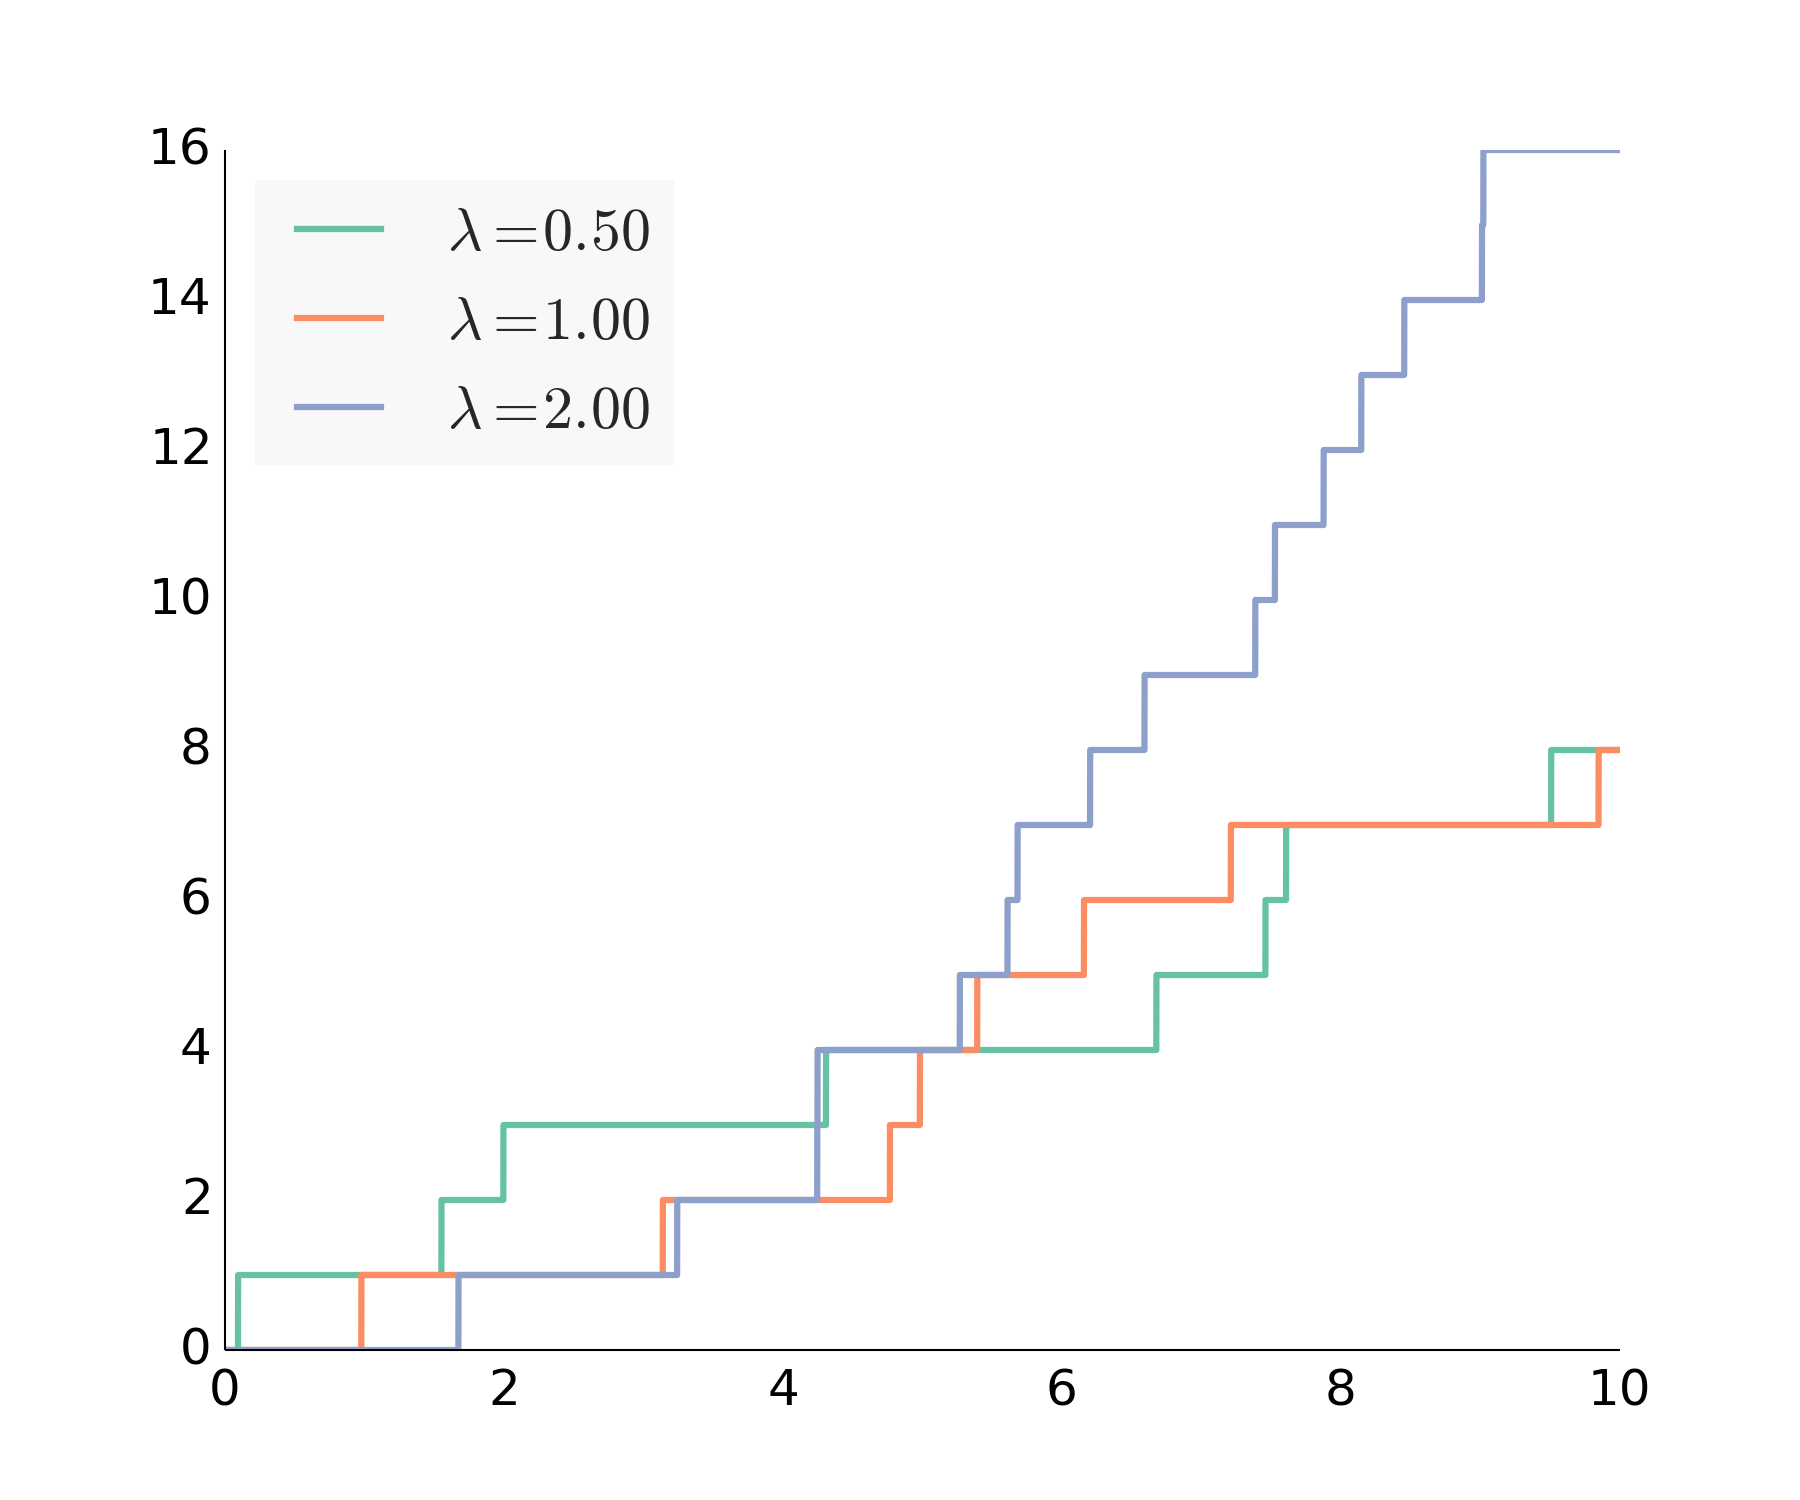
\includegraphics[width=\columnwidth]{figures/figure_2_1.pdf}
\caption[Samples of Poisson Processes.]{Samples of Poisson processes with rates equal to $0.5, 1.0$ and $2.0$.}
\label{fig:poisson_example}
\end{marginfigure}
\par
A doubly stochastic Poisson process, is a process where the rate $\lambda$ is itself a stochastic random variable, usually a function of another stochastic process
$X(t)$. In the case first considered by Snyder, the observations were particle counts of radioactive decay for medical diagnostics. The rate was a function of the 
concentration of the radioactive substance administered to the patient, and by observing particle counts through time onewould like to infer the concentration of 
radioactive substance in the patient's organs. The temporal aspect was relevant because of the fast decay of the radioactive particles. In that case one will have
\begin{subequations}
\begin{equation}
P(N({t+dt})-N(t) = 0 |X(t)) = 1 -\lambda(X(t)) dt + o(dt^2)
\end{equation}
\begin{equation}
P(N({t+dt})-N(t) = 1|X(t)) = \lambda(X(t)) dt + o(dt^2).
\end{equation}
\end{subequations}
The conditional probability of a path $N_{0:t}$ given a path $X_{0:t}$ is then
\begin{equation}
\label{eq:dspp_likelihood}
P(N_{0:t}| X_{0:t}) = \exp\left[ -\int_0^t \lambda(X(s)) ds + \int_0^t \log(\lambda(X(s))) dN(s) \right],
\end{equation}
where I have used the definition of the stochastic integral with respect to a jump process given in \fref{sec:stochastic_proc}.
Defining the jump points $t_i$ as the points where $\lim_{t\downarrow t_i}N(t) \neq \lim_{t\uparrow t_i} N(t)$, one can write the usual formula for the Poisson density of spike times
\[
P(\{t_i\}|X_{0:t}) =   \exp\left[ -\int_0^t \lambda(X(s)) ds \right]\prod_i \lambda(X({t_i})).
\]
Armed with a rate model for the DSPP\marginnote{DSPP: Doubly Stochastic Poisson Process}, one can infer the stimulus history from the count history. The posterior distribution for $X_{0:t}$ is
\begin{equation}
\label{eq:dspp_post}
P(X_{0:t}|N_{0:t}) \propto P(X_{0:t})  \exp\left[ -\int_0^t \lambda(X(s)) ds + \int_0^t \log(\lambda(X(s))) dN(s) \right].
\end{equation}
$P(X_{0:t})$ is a prior distribution over paths of $X(t)$, which in turn are infinite-dimensional objects. This determines the temporal structure of the stimulus, and can be 
tuned to reflect the statistical properties of the stimuli being considered. In practice, it is very hard to compute the full posterior, and for inference purposes, one generally
deals with a  discretised version of the path.\par

Discretising $X_{0:t}$ one can treat the problem of inferring the paths as a multidimensional estimation problem. The simplest way to estimate $X_{0:t}$ is maximum 
likelihood\marginnote{ML = maximum likelihood} whereby one maximises the likelihood given in \fref{eq:dspp_likelihood}. The function given by \fref{eq:dspp_likelihood}
is called a likelihood for $X_{0:t}$ since it does not define a probability density for it. Further, one can incorporate prior beliefs about 
the structure of $X(s)$ by using the full posterior given in \fref{eq:dspp_post}. Taking the value of $X_{0:t}$ that maximises the posterior probability yields the so-called 
\emph{Maximum a Posteriori} estimator.\marginnote{MAP = maximum a posteriori} The full Bayesian approach would be to take the posterior mean as an estimate for 
$X_{0:t}$, that is one takes the mean of the distribution given in \fref{eq:dspp_post} as our estimator. This is usually very hard to compute and has to be done through 
sampling methods.\footnote{For an extensive review of this so-called \emph{decoding} problem see \mycitep{Ahmadian2011,Pillow2011}.}
\par

What if one want to estimate the value of $X(t)$ given $N_{0:t}$ in an online fashion? This corresponds to estimating the marginal probability of $X(t)$ according to
\fref{eq:dspp_post}.
We can derive the results of Snyder informally as follows. Using the same notation as in the Kalman case one has
\[
P(x,t+dt) =\frac{ P\left(X(t+dt)\middle|N_{0:t}\right)P\left(N(t+dt)\middle|X(t+dt)\right)}{P(N(t+dt))}.
\]
When unobserved the distribution of $X$ evolves according to \fref{eq:kolmogorov_fw}. So for infinitesimal $dt$ one can write 
\[
P(X(t+dt)|N_{0:t}) = P(x,t) + \mathcal{A}^\dagger P(x,t) dt.
\]
Furthermore, one can write the quotient of terms dependent on $N(t+dt)$ out as a function of $dN(t)$, leading to
\[
\frac{P(N(t+dt)|X(t+dt),N_{0:t})}{P(N(t+dt))} = (1-dN(t))\frac{1-\lambda(X(t))dt}{1-\hat{\lambda}dt} + dN(t)\frac{\lambda(X(t))}{\hat{\lambda}},
\]
where $\hat{\lambda} = \int dx P(x,t) \lambda(x)$. Expanding and discarding terms of order $dt^2$ and $dN(t)dt$, yields
\[
\frac{P(N(t+dt)|X(t+dt),N_{0:t})}{P(N(t+dt))} = 1-dN(t) -\lambda(X(t))dt +\hat{\lambda}dt +dN(t)\frac{\lambda(X(t))}{\hat{\lambda}},
\]
which rearranging terms, can be written as
\[
\frac{P(N(t+dt)|X(t+dt),N_{0:t})}{P(N(t+dt))} = 1 + \left(\lambda(X(t))-\hat{\lambda}\right)\hat{\lambda}^{-1}\left(dN(t)-\hat{\lambda} dt\right).
\]
Inserting this into the relation above gives
\[
P(x,t+dt) = P(x,t) +\mathcal{A}^\dagger P(x,t) dt + P(x,t)\left(\lambda(x)-\hat{\lambda}\right)\hat{\lambda}^{-1}\left(dN(t)-\hat{\lambda} dt\right),
\]
or, writing it as a stochastic PDE,
\begin{equation}
\label{eq:snyder_uni}
d_t P(x,t) = \mathcal{A}^\dagger P(x,t) dt + P(x,t)\left(\lambda(x)-\hat{\lambda}\right)\hat{\lambda}^{-1}\left(dN(t)-\hat{\lambda} dt\right).
\end{equation}
Note the striking similarity with \fref{eq:kushner}, namely the observations only influence the posterior through an innovation process, here given by $dN(t)-\hat{\lambda}dt$. Furthermore, the inverse rate is equivalent to the inverse variance, since the variance of a Poisson process is precisely its rate $\lambda(x)$. This equation was first derived by Donald Snyder in 1972.\mycite{Snyder1972}
\par
Clearly the derivation above is not mathematically sound. More care is needed when taking limits with $dt\to 0$, namely I have ignored the terms of order $dN(t) dt$ 
in \fref{eq:snyder_uni}. This can be shown to be rigorous, but is beyond the scope of this thesis.\footnote{See \mycitep{privault2014} for a full introduction to the stochastic
calculus of jump processes.} The full derivation by Snyder first finds an expression for the 
characteristic function of the posterior distribution and then derives a stochastic PDE for the characteristic function. This is then Fourier-transformed to yield 
\fref{eq:snyder_uni}.

\subsection{Multiple Spike Trains}

\Fref{eq:snyder_uni} is readily extended to multiple point processes, as long as they are independent. Given a population of point processes $N^i(t)$, $i\in [1,M]$, one will simply have, following the same derivation
\begin{equation}
\label{eq:snyder_multi}
d_t P(x,t) = \mathcal{A}^\dagger P(x,t) dt + P(x,t)\sum_i\left(\lambda_i(x)-\hat{\lambda}_i\right)\hat{\lambda}_i^{-1}\left(dN^i(t)-\hat{\lambda}_i dt\right).
\end{equation}
Again, this can be be compared with a multidimensional observation process in the Kalman case by noting that one can rewrite it as
\begin{equation}
\nonumber
d_t P(x,t) = \mathcal{A}^\dagger P(x,t) dt + P(x,t)\left(\boldsymbol{\lambda}(x)-\hat{\boldsymbol{\lambda}}\right)^\top Diag(\hat{\boldsymbol{\lambda}})^{-1}\left(d\boldsymbol{N}(t)-\hat{\boldsymbol{\lambda}} dt\right).
\end{equation}
I have used the notation $\boldsymbol{\lambda}(x) = (\lambda_1(x),\lambda_2(x),\ldots)^\top, d\boldsymbol{N}(t) = (dN^1(t), dN^2(t),\ldots)^\top$ and so forth. Note that, taking the
vector counting process $\boldsymbol{N}(t)$, its covariance will be $Diag(\hat{\boldsymbol{\lambda}})$, and the equation corresponds precisely to \fref{eq:kushner}.

\section{Fast Population Coding and Dense Tuning Functions}

\label{sec:fast_coding}

A similar filtering framework was proposed in the computational neuroscience community as well.\mycite{Huys2007} The main question being asked was how one can extend the 
framework of population coding, which usually relied on cumulative rates, to coding in a short-time regime. Filtering from spike trains has also been of central importance to the study of 
Brain-Computer-Interfaces, where one tries to decode intended movements or actions from the activity of neurons in the brain.\mycite{Ergun2007} One issue that is central in the 
approach of \mycitet{Huys2007} is the assumption that the population firing rate is independent of the stimulus. I will first extend \fref{eq:dspp_likelihood} to multiple independent Poisson 
processes. This yields
\begin{equation}
\label{eq:dspp_multi_likelihood}
P(\{N^i_{0:t}\}|X_{0:t}) = \exp\left[\sum_i \int \log(\lambda_i(X(s)))dN^i(s) -\int \lambda_i(X(s))ds\right].
\end{equation}
If the tuning functions are distributed such that $\sum_i\lambda_i(X) = C$, irregardless of $X$, this can be simplified substantially. This is the same as saying that the process 
$N(t) = \sum_i N^i(t)$ is a homogeneous Poisson process with rate $C$.
One will then have
\begin{equation}
P(\{N^i_{0:t}\}|X_{0:t}) \propto \prod_i \exp\left[\sum_i \int \log(\lambda_i(X(s))) dN^i(s)\right].
\end{equation}
The integral with respect to $dN^i(s)$ will only yield non-zero terms where $N^i(t)$ is discontinuous, therefore the resulting term will be simply a product of the rates of the neurons at the times they spiked. Let us denote the set of spikes emitted by the population by $\boldsymbol{S}(t) = \{(n_i,t_i)\}_{i=1}^{N(t)}$, where $n_i$ denotes the identitiy of the $i$-th neuron to spike and $t_i$ denotes its spike time. One can then write
\begin{equation}
P(\{N^i_{0:t}\}|X_{0:t}) \propto \prod_{\boldsymbol{S(t)}} \lambda_{n_s}(X(t_s)).
\end{equation}
Furthermore, assume that the the tuning functions $\lambda_i$ are unnormalized Gaussians of the form
\begin{equation}
\label{eq:dense_poiss_gauss_tf}
\lambda_i(x) = \phi \exp\left[-\frac{1}{2} (x-\theta_i)^\top \covar^\dagger (x-\theta_i)\right],
\end{equation}
where I have used the pseudoinverse $\covar^\dagger$ to allow for the tuning functions to be degenerate Gaussian distributions. This poses no problem, as the prior 
over $X(t)$ will be chosen to be Gaussian, leading to a Gaussian posterior when multiplied by $\lambda_i/\hat{\lambda}_i$.
Furthermore the marginal rate of a spike being fired $\hat{\lambda}_i = \boldsymbol{E}_X\left[\lambda_i(x)\right]$ is also 
defined. One must note that $\lambda_i$ does not define a distribution over the stimulus space but a rate of arrival of observations. The Gaussian updates are, however 
the same.\par

I can now treat the problem similarly to the Kalman filter problem, but one needs to take into account the fact that instead of arriving continuously, observations are coming in at random 
times. Consider the same process as before given by the SDE
\[
dX(t) = AX(t) dt + H^{1/2} dW(t).
\]
In the absence of observations the Gaussian distribution will evolve as
\begin{subequations}
\label{eq:free_ou_moments}
\begin{equation}
\frac{d\mu}{dt} = A \mu
\end{equation}
and
\begin{equation}
\frac{d\Sigma}{dt} = A\Sigma + \Sigma A^\top + H.
\end{equation}
\end{subequations}
Therefore, the posterior distribution over $X(t)$ between observations is given by $\mathcal{N}(\mu(t),\Sigma(t))$.
If a neuron with tuning centre $\theta_i$ spikes at time $t$, the posterior density will be updated by
\[
P(X(t)|\textrm{spike}) =\frac{\lambda(X(t)) \mathcal{N}(\mu(t),\Sigma(t))}{\hat{\lambda}}.
\]
Completing squares in the exponents, one obtains for the posterior mean
\begin{subequations}
\label{eq:gaussian_updates}
\begin{eqnarray*}
\mu(t) =&  \left(\Sigma(t^-)^{-1} + \covar^\dagger\right)^{-1} \left(\Sigma(t^-)^{-1} \mu(t^-) + \covar^\dagger \theta_i\right)\\
=&\mu(t^-) -\left(\Sigma(t^-)^{-1} + \covar^\dagger\right)^{-1}\left(\Sigma(t^-)^{-1} + \covar^\dagger\right)\mu(t^-)\\
+&\left(\Sigma(t^-)^{-1} + \covar^\dagger\right)^{-1} \left(\Sigma(t^-)^{-1} \mu(t^-) + \covar^\dagger \theta_i\right),
\end{eqnarray*}
and finally
\begin{equation}
\mu(t) = \mu(t^-) + \Sigma(t)^{-1} \covar^\dagger\left(\theta_i - \mu(t^-)\right).
\end{equation}
For the covariance one has
\begin{eqnarray*}
\Sigma(t) =& \left(\Sigma(t^-)+\covar^\dagger\right)^{-1}\\
=& \Sigma(t^-) -\Sigma(t^-)\left(\Sigma(t^-)+\covar^\dagger\right) \left(\Sigma(t^-)+\covar^\dagger\right)^{-1}+\left(\Sigma(t^-)+\covar^\dagger\right)^{-1},
\end{eqnarray*}
yielding
\begin{equation}
\Sigma(t) = \Sigma(t^-) - \Sigma(t^-) \covar^\dagger \Sigma(t^-) \left(I+\covar^\dagger \Sigma(t^-)\right)^{-1}.
\end{equation}\marginnote{These updates can be simplified if the tuning matrix $E$ is invertible.}
\end{subequations}
These equations can be condensed into SDE's for the posterior mean and covariance very simply. The mean will be given by
\begin{subequations}
\label{eq:filtering_sdes}
\begin{equation}
d\mu(t) = A\mu(t) dt + \sum_i dN^i(t) \left[\Sigma(t^-)\left(I+\covar^\dagger \Sigma(t^-)\right)^{-1} \covar^\dagger\left(\theta_i - \mu(t^-)\right)\right]
\end{equation}
and the covariance by
\begin{equation}
\label{eq:filtering_sde_sigma}
d\Sigma(t) = (A\Sigma(t) + \Sigma(t) A^\top+H)dt + dN(t) \left[\Sigma(t^-) \covar^\dagger \Sigma(t^-) \left(I+\covar^\dagger \Sigma(t^-)\right)^{-1}\right].
\end{equation}
\end{subequations}
These SDE's define processes that are continuous from the right and have a limit from the left. They are often called C\`adl\`ag processes in the stochastic literature, 
from the french phrase \emph{continue \`a droite, limite \`a gauche}. The evolution of the posterior variance only depends on the total spike count process 
$N(t)$, which will be fundamental for the future analysis.
\par

As I mentioned before, the covariance of the tuning functions does not need to be invertible. Note that as long as $\Sigma(t)^{-1} + \covar^\dagger$ is invertible, the 
filtering 
equations are always well-defined. This can be ensured by requiring that $E$ be positive semidefinite. Since $\Sigma(t)$ is positive definite, as it 
is a covariance matrix, $\Sigma(t)^{-1}+\covar^\dagger$ will also be positive definite.
\par

Most of the analytic work in this thesis is done on the filtering problem given by \fref{eq:filtering_sdes}. The fact that the total frequency of observations is independent of 
the system's state along with the homogeneous nature of the population of processes leads to a number of simplifications when evaluating the
Mean-Squared-Error\marginnote{Mean-Squared-Error $\equiv$ MSE} of the estimator $\mu(t)$. More specifically, since $\mu(t)$ is the posteriori mean estimator, its MSE is 
given by the average posterior variance.\footnote{This will be shown in the beginning of \fref{chap:mse}.}
The filtering scheme described in this section and some of the results of \fref{chap:mse} are illustrated in \fref{fig:matern_coding}.
\begin{figure}
\label{fig:matern_coding}
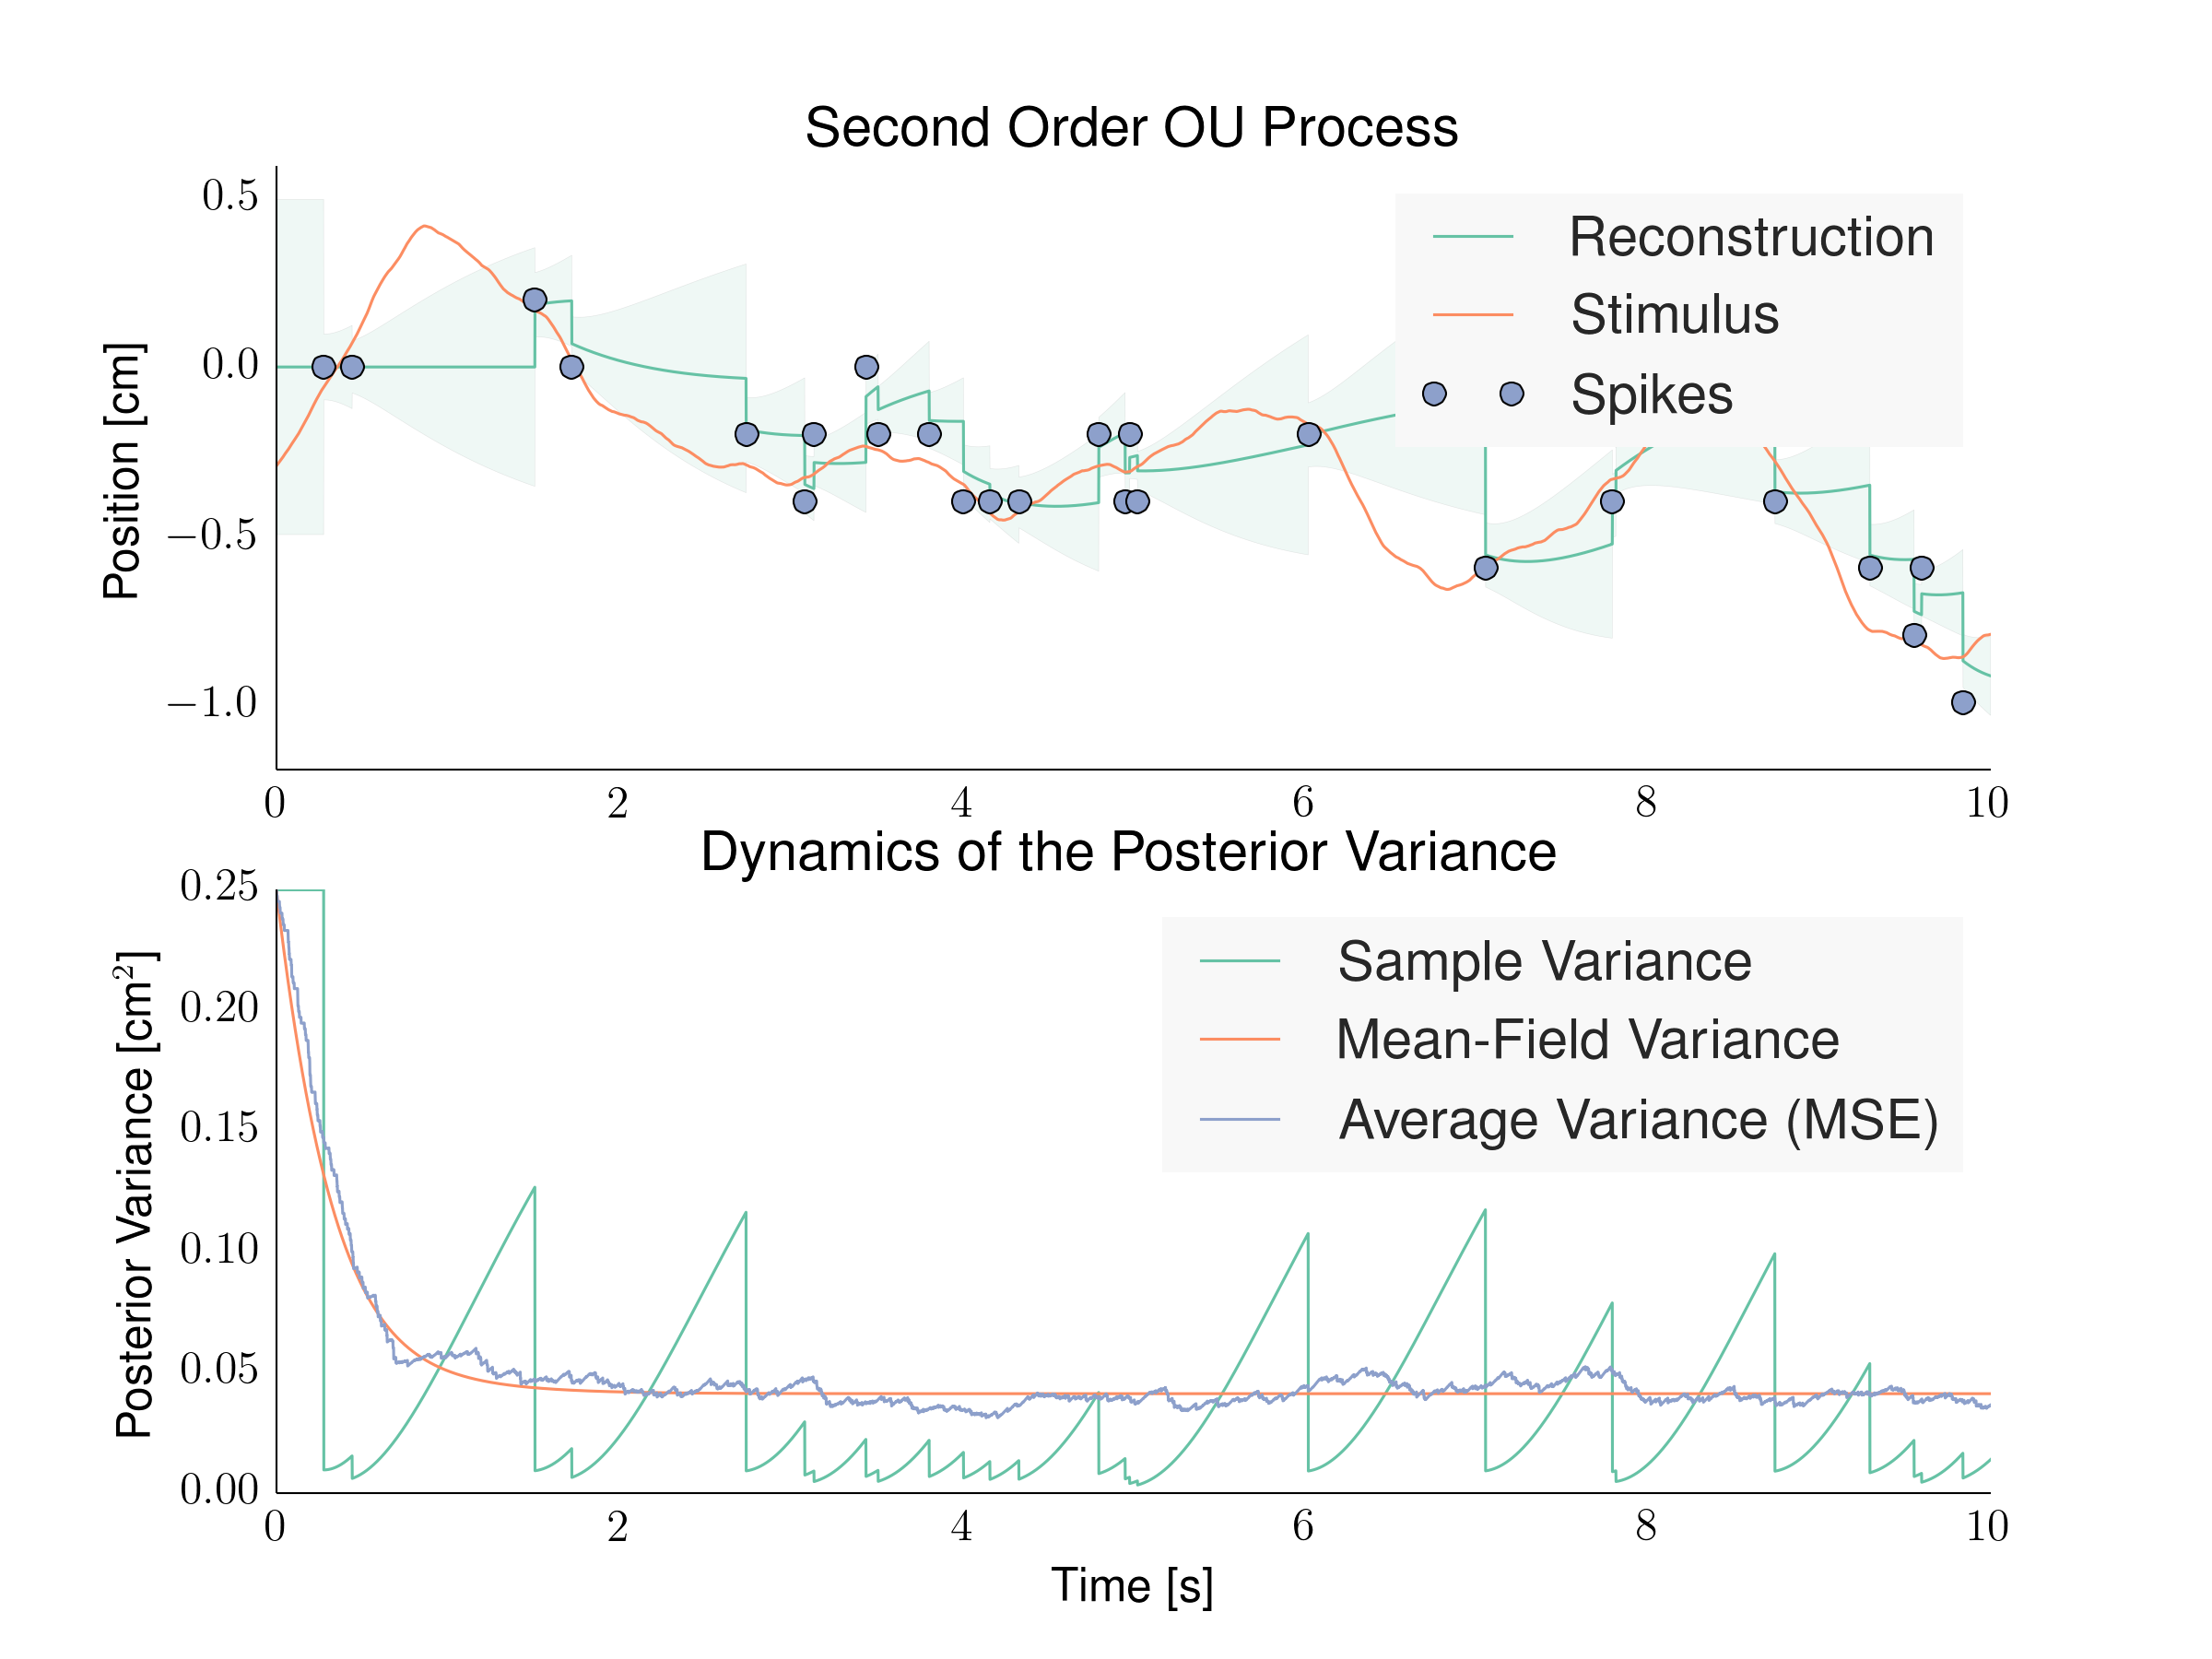
\includegraphics[width=\columnwidth]{figures/figure_2_2.pdf}
\caption[Online decoding of a spike train.]{The general filtering framework: the unobserved process we are trying to estimate is shown as the solid red line, while the observed spikes are
shown as red dots, aligned by the preferred stimulus of the firing neurons. The posterior mean estimate is given by the dotted blue line, while the light red shading
gives the confidence interval of one standard deviation. Note the discontinuous jumps in the mean and covariance at the times of spikes. The lower figure shows the
average posterior variance over all possible spike trains given a stimulus distribution. Note that the mean-field approximation provides a very good account of the
evolution of the average. These results will be further discussed in \fref{chap:mse}.}
\end{figure}

I will now turn to filtering from Point processes when the dense coding assumption does not hold.

\section{Methods for General Filtering of Point Processes}

If nothing else is known about the process at hand, one is forced to work directly with \fref{eq:snyder_multi}. In principle one could discretise the state space and try to 
solve the Partial Differential Equation\marginnote{Partial Differential Equation $\equiv$ PDE} recursively as the observations come in. In practice, however, 
the right hand side \fref{eq:snyder_multi} also contains averages over $P(x,t)$, leading to additional complications on every integration step. One way to circumvent this 
particular problem is to work with unnormalized probabilities. The Zakai equation\mycite{Zakai1969} is a modified version of the Kushner equation which propagates 
unnormalized probabilities. For a stochastic process $X(t)$ observed through another process $Y(t)$ as given in \fref{sec:kalman}, one can define $\rho(x,t)$ as a solution to
\begin{equation}
\label{eq:zakai}
d_t\rho(x,t) = \mathcal{A}^\dagger \rho(x,t) dt+ \rho(x,t) x^\top C^\top D dY(t),
\end{equation}
with $\rho(x,0) = P_0(x)$. It can then be shown that $P(x,t) = \rho(x,t)/\int dx \rho(x,t)$.
Any solution to the Zakai equation will yield a solution to the corresponding Kushner equation when normalised.
Note that, while the Kushner equation was a stochastic partial integro-differential equation, since the left hand side involved averages over $P(x,t)$, the Zakai equation is 
a simpler linear stochastic partial differential equation and given a realisation of the observation process can be solved by standard PDE methods.
%Furthermore, the Zakai equation allows for a closed form solution in terms of path integrals.
\par
I will present a similar framework for the Snyder equation \ref{eq:snyder_uni}. Again taking the notation $P(x,t) = \rho(x,t) / \int dx \rho(x,t)$ one finds that the 
unnormalised posterior distribution $\rho(x,t)$ of a stochastic process with generator $\mathcal{A}$ observed through a doubly stochastic Poisson process with 
rate 
$\lambda(x)$ will obey the stochastic PDE
\begin{equation}
\label{eq:zakai_snyder}
d_t\rho(x,t) = \mathcal{A}^\dagger \rho(x,t) dt -\lambda(x) \rho(x,t) + \left(\lambda(x) -1 \right)\rho(x,t) dN(t).
\end{equation}
Note that any term independent of $x$ can be trivially discarded as it only constitutes a temporal renormalisation of $\rho$. For example, if $\rho^*(x,t)$ is a solution to
\fref{eq:zakai_snyder} with initial condition $\rho(x,0) = g(x)$, then $r(x,t) = \exp\left(-\int_0^t k(s) ds ) \rho^*(x,t)\right)$ is a solution to the stochastic PDE
\[
d_t r(x,t) = \mathcal{A}^\dagger r(x,t) dt -\lambda(x) r(x,t) + \left(\lambda(x) -1 \right) r(x,t) dN(t) -k(t) r(x,t) dt,
\]
with the same initial condition.
This allows one to set a baseline to the expected firing rate in the unnormalised equation. This framework has been used by \mycitep{Bobrowski2009} in
the study of finite state systems observed through doubly stochastic Poisson processes. This work was also extended to static continuous processes by 
Yaeli and Meir.\mycite{Yaeli2010}. I will now discuss the application of these equations to the development of a particle filter for the filtering problems discussed above.


\subsection{Particle Filtering}

The central idea of particle filtering is relatively simple. If one is not given access to the system's state directly, one can just simulate a large number of hypotheses of 
the  system's state and weight each copy according to its agreement with the observations. One can then compute averages over the posterior distribution from the 
weighted samples. Say I have a system with state $X(0)$ initially distributed according to $P_0(x)$, some known transition probability 
\[
W(x,x') \equiv P_{X(t)}\left(x\middle|\,X(t)=x'\right),
\]
and I am given observations of a second process $Y(t)$, with probability density 
\[
\mathcal{L}(y,x) \equiv P_{Y(t)}\left(y\middle|\,X(t)=x\right).
\]
If all the probabilities are known I can implement the filtering  steps numerically,
by taking a sample of $M$ \emph{particles} $\{Z^i(0)\}, i \in [1,\ldots,M]$ from $P_0(x)$, and associating a weight to each of those 
particles $w^i(0)= 1$. Then for each 
particle $Z^i$ I sample the state of that particle at the following instant through the transition probability 
\[
P_{Z^i(t)}(z|Z^i(t-dt)) = W(z,Z^i(t-dt))
\]
and reweigh it through the likelihood
of $Y(t)$, yielding 
\[
w^i(t) = w^i(t-dt) \mathcal{L}(Y(t),Z^i(t)).
\]
The approximate density $Q(x,t) = \sum_i w^i(t)\delta(Z^i(t) - x)/\sum_i w^i(t)$, then gives an 
approximation of the
posterior density $P(x,t)$ and averages can be computed by simply aggregating over the particles, giving
\[
\int dx\, P(x,t) g(x)  \approx \int dx\, Q(x,t) g(x)  = \frac{1}{\sum_i w^i(t) }\sum_i w^i(t) g(Z^i(t)).
\]
These methods are often called Sequential Monte Carlo\marginnote{SMC: Sequential Monte Carlo} methods, since they consist of sequentially sampling the 
state of the system in a way similar to a Monte Carlo Markov Chain.
\par

The description above barely scratched the surface of what is achievable and what are the problems of particle filters, and I will not dive too deeply into the theory of
them, but one point should be made. Though the sampling procedure described above in principle yields an estimate of the true posterior distribution, a lot can
go wrong when implementing it with a finite number of particles. One issue that plagues many such filters is the issue of weight depletion. Weight depletion refers
to the situation where all but a few particles have very low weights, representing state paths which are incompatible with the observations. This can lead the particle
filter to waste resources estimating the density of regions which don't contribute to the posterior averages, and therefore yielding very poor estimates of the distribution
in the interesting regions. This led researchers to propose resampling steps in the particle filter. Whenever a certain criterion is met (or after every step in the filter) one 
can resample the particles from the set of existing particles according to their weights, i.e., sample $M$ particles from the set $\{Z^i(t)\}$ with probabilities given by
$p_i = w^i(t)/\sum_i w^i(t)$. After that, all weights are reset to 1 and the procedure continues. This forces
the filter to allocate its particles according to its current estimate of the posterior distribution, preventing weight depletion to some extent. It is not a panacea for these 
issues, however, and even properly resampled filters can often end up with very poor estimates of the posterior distribution.
\par

Another important thing to note, is that it is often not possible to efficiently sample from the transition probabilities of the system. In those cases one can still combine
the particle filter with an importance sampling approach. In that sense, at every step one samples from a simpler distribution $Q(Z^i(t)|Z^i(t-dt))$ and reweighs the 
particles according to 
\[
w^i(t) = w^i(t-dt) \frac{P(Y(t) | Z^i(t)) P(Z^i(t)|Z^i(t-dt))}{Q(Z^i(t)|Z^i(t-dt))}.
\]
This allows for efficient sampling, but it adds another source of
weight depletion. Again, if the sampling transition probabilities do not match the system's transition probabilities, the weights will quickly fall to low values, leading to
poor estimates of the posterior distribution.
\par

Let us consider again the general case of doubly stochastic Point process filtering. Note that in the absence of spikes the posterior evolves according to
\begin{align*}
\frac{\partial P(x,t)}{\partial t} =& \mathcal{A}^\dagger P(x,t) + (\hat{\lambda}(t) - \lambda(x,t) ) P(x,t).
\end{align*}
For linear diffusion processes, this simplifies to
\begin{align}
\label{eq:particle_fokkerplanck}
\frac{\partial P(x,t)}{\partial t} =& -\nabla \cdot \left(Ax P(x,t)\right) + \frac{1}{2}\Tr\left[ H \frac{\partial^2 P(x,t)}{\partial x_i\partial x_j}\right]+ (\hat{\lambda}(t) - \lambda(x,t) ) P(x,t).
\end{align}
I can again define an unnormalised density $\rho(x,t)$ evolving according to
\[
\frac{\partial \rho(x,t)}{\partial t} =-\nabla \cdot \left(Ax P(x,t)\right) + \frac{1}{2}\Tr\left[ H \frac{\partial^2 P(x,t)}{\partial x_i\partial x_j}\right] -\lambda(x,t) \rho(x,t),
\]
for which the normalised density $\rho(x,t) / \int dx \rho(x,t)$ satisfies \fref{eq:particle_fokkerplanck}.
It can be shown that the equation above describes the evolution of a drift diffusion process with a death rate of $\lambda(x,t)$. This means that the system evolves
according to the \fref{eq:OU_sde} but there is a transition to a death state with a rate $\lambda(x,t)$.\mycite{Oksendal2003} This allows one to formulate a simple particle 
filter, by propagating the particles with the transition probability of the linear stochastic system and then killing it at a rate $\lambda(Z^i(t),t)$, resampling the particles every
time a particle \emph{dies}. Alternatively one can reweigh the weights according to $1-\lambda(Z^i(t),t)dt$ after every time step, obtaining the same effect.
\par
The particle filtering scheme presented here is very flexible, and is in principle applicable to any kind of stochastic process observed through Poisson spikes. This
approach has also gained traction in the neuroscience community, where particle filters are often used to decode cortical signals from electrophysiological
recordings.\mycite{brockwell2004recursive,Ergun2007} Most BCI application require very low latency though, and often specialised types of Kalman filter are more practical to employ in such settings.\mycite{wu2006bayesian}

\subsection{Assumed Density Filtering}

\label{sec:ADF}

Though the presented framework of DSPP's in dense Gauss-Poisson populations of neurons turns out to be exactly Gaussian, this does not hold generally. For example,
one could have a stimulus-dependent population firing rate, leading to non-Gaussian posteriors. One would
then have to deal with the full extent of the Snyder \fref{eq:snyder_multi}. One way to deal with this is to project the posterior distribution to a Gaussian at every time step, that is, at every time
$t$, one looks at the resulting distribution at the next time step $t+dt$ and approximates it with a Gaussian. To do
so one needs to determine the mean and covariance of the posterior and can then match a Gaussian distribution to those moments. 
\par

This approach is usually called Assumed Density Filtering\marginnote{ADF: Assumed Density Filtering}. Given some variable of interest $x$ and a set of observations of random 
variables $\{Y_1,\ldots, Y_N\}$ distributed as $P_Y(y|x)$, ADF consists of sequentially incorporating the observations and
finding the best approximation to the posterior within a family of distributions. For example, if the true, intractable distribution were $P(x|Y_1,\ldots,Y_N)$ one
could choose to approximate it by a Gaussian distribution. One would start out with a prior distribution $Q_0(x)$ and sequentially look
for the best Gaussian approximation to the posterior $Q_i(x) P(Y_{i+1}|x)$. This is usually termed filtering even when there is no temporal estimation
involved because of the sequential updates to the posterior.\footnote{For examples of applications, see \mycitep{opper1998,boyen1998,minka2001}.} The best
approximation to the posterior is usually defined as the one minimising the Kullback-Leibler divergence between the full and approximate posterior. In that sense,
given a current approximation $Q_i(x)$ and a new observation $Y_{i+1}$, the update to our approximate posterior would be
\begin{align*}
Q_{i+1} (x) =& \argmin_q KL[Q_i(x) P(Y_{i+1}|x)||q] \\=& \argmin_q \int dx\, Q_i(x) P(Y_{i+1}|x) \log \frac{Q_i(x) P(Y_{i+1}|x)}{q(x)}.
\end{align*}
The KL divergence taken here is the reverse of the KL divergence used in variational inference.\footnote{In variational inference one usually considers
the KL divergence between the approximating and the true distribution given by $KL[q||p] = \int dx q(x) \log\frac{q(x)}{p(x)}$. When $q(x)$ is tractable or allows for
exact integration, this allows for simplifications of the KL-divergence.} It can be shown that if one applies this 
process using a family of exponential distributions as approximating distributions, it will lead
to a moment matching procedure where the moments of the approximating distribution match the ones of the posterior $Q_i(x) P(Y_{i+1}|x)$.\footnote{See \fref{app:moment} for a 
short 
clarification.} If one took $Q(x)$ to be a Gaussian in every step, the procedure would involve evaluating the mean and covariance of the posterior and setting the new distribution to a 
Gaussian with that mean and covariance.
\par

A simple example of a factor leading to a non-Gaussian posterior in the filtering problem described in this chapter is the presence of adaptation in the firing rates. Poisson processes 
are memoryless,
that is, the probability of a spike being fired is independent of the time since the last spike. It is well known, however, that biological neurons do not follow that rule. For example,
there is a clear refractory period in action potential generation, rendering a neuron incapable of firing an action potential for a short period after the firing of an action potential, 
regardless of the stimulation applied. This
refractory period varies from cell type to cell type and between organisms, but is generally around 5 ms. Another very common phenomenon is
spike-frequency-adaptation,\mycite{benda2003} where upon continued stimulation a neuron reduces its frequency from its initial response frequency to a lower frequency.
A simple Poisson process can not account for these phenomena, but it is easy to modify the Poisson model to account for a refractory period or else to include a spike-frequency 
adaptation component as well.
\par

Consider a simple history-dependent Poisson process given by a rate $\lambda(x,t) = \kappa(t) \lambda(x)$, where $\kappa$ itself depends on the
spiking history of the process. Let me take $\kappa$ evolving according to the SDE
\[
d\kappa(t) = \frac{(\phi - \kappa(t))}{\tau} dt - h(\kappa(t)) dN(t), \quad h(\kappa) = \min(\Delta, \kappa),
\]
where $dN(t)$ is the spike train of the neuron.
This will lead to a rate modulation which stabilises at $\phi$ when there are no spikes, and is shifted downwards by $\Delta$ whenever there is a spike, without
venturing below 0. Although the process is now history-dependent, the joint process $\kappa(t),N(t)$ is still Markov, since the dynamics of $\kappa$ itself
is Markovian. This allows one to model a neuron with a refractory period by taking a relaxation time $\tau \approx 5 ms$ or to model a neuron with spike-frequency-adaptation by taking longer relaxation times.\par

The filtering probability for a diffusion process observed through a population of adaptive neurons with rates given by $\lambda^i(x,t) = \kappa^i(t) \lambda^i(x)$ is given by
\begin{equation}
\label{eq:snyder_adf}
d_t P(x,t) = \mathcal{A}^\dagger P(x,t) dt + P(x,t)\sum_i\left(\lambda_i(x,t)-\hat{\lambda}_i(t)\right)\hat{\lambda}_i(t)^{-1}\left(dN^i(t)-\hat{\lambda}_i(t) dt\right),
\end{equation}
which is \fref{eq:snyder_uni} with time-dependant firing rates. One now needs to integrate the set of equations for the rate modulations $\kappa^i(t)$ for every neuron as well, to be 
able to solve the Snyder equation properly.
\par

The ADF approach for this case would work as follows: one starts out with an initial Gaussian distribution $\mathcal{N}(\mu(0),\Sigma(0))$ at $t=0$; then, for every instant $t$ one 
determines the non-Gaussian probability P(x,t+dt) at the next instant $t+dt$ via \fref{eq:snyder_adf}; after that, one finds the mean and covariance of $P(x,t+dt)$, and approximates the 
distribution by a Gaussian with the same mean and covariance and proceeds to the next instant. This can be cast into a set of differential equations and updates governing the
mean and covariance of our approximate posterior.
\par

To obtain the ADF equations for this simple model I need to evaluate the evolution of the mean and covariance of the filtering distribution. I will derive the
necessary equations similarly to the derivation of the differential Chapman-Kolmogorov equation in \mycitep{Gardiner2004}.The average of
a function of $x$ over the posterior distribution evolves as
\begin{align*}
\frac{\partial \boldsymbol{E}_P[f]}{\partial t} = \frac{\partial \int dx f(x) P(x,t)}{\partial t} = \lim_{dt\to 0} \frac{\int dx f(x) \left(P(x,t+dt)-P(x,t)\right)}{dt}.
\end{align*}
In the absence of spikes, the limit can be evaluated, as all terms are of order $dt$, obtaining
\begin{align*}
\frac{\partial \boldsymbol{E}_P[f]}{\partial t} =& \int dx f(x) \left(\mathcal{A}^\dagger P(x,t) + (\hat{\lambda}(t) - \lambda(x,t) ) P(x,t)\right) \\
=&\int dx  P(x,t) \left(\mathcal{A} f(x)+ f(x) (\hat{\lambda}(t) - \lambda(x,t) ) \right).
\end{align*}
This can be readily cast into a form to allow for moment matching of Gaussian distributions. Taking a stochastic process $X(t)$ given by the SDE
\[
dX(t) = A\left(X(t)\right) dt + H\left(X(t)\right)^{1/2} dW(t),
\]
the infinitesimal generator and its adjoint will be given by
\[
\mathcal{A} f = A(x)^\top \nabla f(x) +  \frac{1}{2}\Tr\left[H(x) \frac{\partial^2 f(x)}{\partial x^2}\right],
\]
and
\[
\mathcal{A}^\dagger f = -\nabla \cdot\left(A(x) f(x)\right) + \frac{1}{2}\Tr\left[ \frac{\partial^2 H(x) f(x)}{\partial x^2}\right].
\]
The evolution of the mean and covariance will thus be given by
\begin{subequations}
\begin{equation}
\frac{\partial \mu(t)}{\partial t } = \boldsymbol{E}\left[A(x)\right] + \boldsymbol{E}\left[x \left(\hat{\lambda}(t) -\lambda(x,t)\right)\right],
\end{equation}
\begin{align}
\frac{\partial \Sigma(t)}{\partial t} = &\boldsymbol{E}\left[A(x)(x-\mu(t))^\top\right] + \boldsymbol{E}\left[(x-\mu(t)) A(x)^\top\right] + H(x)\nonumber\\ +&\boldsymbol{E}\left[(x-\mu(t)) (x-\mu(t))^\top \left(\hat{\lambda}(t) -\lambda(x,t)\right)\right].
\end{align}
\end{subequations}
These equations are exact, even if the posterior distribution is not Gaussian. If the posterior is Gaussian, the averages on the right hand side of these equations can be 
written as a function of $\mu(t)$ and $\Sigma(t)$, therefore providing a closed system for the evolution of these variables. The crucial step to perform ADF is to assume that the 
distribution at every
instant is characterised by only its mean and covariance, and is therefore Gaussian. In that case, the averages in the equations can often be performed exactly and 
one can provide an approximate filter to the problem. Note that the derivation is valid for the case of multiple spike trains as well, yielding
\begin{subequations}
\label{eq:adf_gauss_filter}
\begin{equation}
\frac{\partial \mu(t)}{\partial t } = \boldsymbol{E}\left[A(x)\right] + \sum_i\boldsymbol{E}\left[x \left(\hat{\lambda}^i(t) -\lambda^i(x,t)\right)\right],
\end{equation}
\begin{align}
\frac{\partial \Sigma(t)}{\partial t} = &\boldsymbol{E}\left[A(x)(x-\mu(t))^\top\right] + \boldsymbol{E}\left[(x-\mu(t)) A(x)^\top\right] + H(x)\nonumber\\ +&\sum_i\boldsymbol{E}\left[(x-\mu(t)) (x-\mu(t))^\top \left(\hat{\lambda}^i(t) -\lambda^i(x,t)\right)\right].
\end{align}
\end{subequations}\par

In \fref{chap:optimal} I will apply the ADF approach to the general linear stochastic systems considered here as well as a nonlinear stochastic system and compare 
them to the particle filter approach. 
Though the ADF has had considerable success and has spawned a number of new approaches, most notably the expectation propagation (EP)
algorithm,\mycite{opper2000,minka2001} the theoretical guarantees of particle filters have led me to prefer it when estimating the MSE of an approximate filter.

\section{Filtering for General Gaussian Processes}
\label{sec:gp_filtering}
The linear stochastic processes I have considered in this chapter are special cases of Gaussian Processes. A Gaussian Process is a process $X(t)$ such that the 
marginal distribution of the process at a set of times $\{t_1,\ldots,t_M\}$ is always given by a Gaussian distribution. Furthermore, the density of $X(t)$ at said points
is given by
\[
P\left(X(t_1),X(t_2),\ldots,X(t_m)\right) = \mathcal{N}\left((m(t_1),m(t_2),\ldots,m(t_M))^\top, K(t_i,t_j)\right), \textrm{ where } 1\le i\le M, \quad 1\le, j \le M.
\]
The covariance of a GP\marginnote{GP $\equiv$ Gaussian Process} is given by the kernel function $K(s,t)$, which specifies the temporal structure of the process at 
hand. It is straightforward to show that the unobserved Ornstein-Uhlenbeck process
\[
dX(t) = -\gamma X(t) dt + \sigma^{1/2} dW(t),
\]
describes a Gaussian process with zero mean and kernel $K_{OU} (s,t) = \frac{\sigma}{2\gamma} e^{-\frac{|t-s|}{2\gamma}}$.\par

Gaussian Processes have become a very popular method in Machine Learning, as they allow one to specify a distribution of random functions over a
domain.\mycite{Rasmussen2005}
\par

Assume one is trying to estimate a function $f(t)$ drawn from a GP prior with zero mean and kernel $k(s,t)$. If one is given $M$
observations $(t_i,y_i)$ of the value of $f$ at times $t_i$, one can write the marginal distribution of $f(t)$ for any time $t$ by simple manipulation of Gaussian densities.
If the observations are corrupted with Gaussian noise with variance $\alpha^2$, the probability density of the observations is given by
\[
P(y_1,\ldots,y_M) = \mathcal{N} (\boldsymbol{0},K(t_i,t_j)+\alpha^2 \delta_{i,j}), \textrm{ where } 1\le i\le M, \quad 1\le, j \le M.
\]
The joint density of $f(t)$ and the observations is given by
\[
P(f(t),y_1,\ldots,y_M)= \mathcal{N} \left(\boldsymbol{0},\left[\begin{array}{cc} K(t,t) & K(t,t_i)\\K(t,t_j)& K(t_i,t_j)+\alpha^2\delta_{i,j}\end{array}\right]\right).
\]
Let $G_{i,j} = K(t_i,t_j)$, $\boldsymbol{y} = (y_1,\ldots,y_M)^\top$ and $k(t,\{t_i\}) = (K(t,t_1),\ldots,K(t,t_M))^\top$.
The conditional distribution of $f(t)$ given the observations can then written as
\[
P(f(t)|y_1,\ldots,y_M) =\mathcal{N}\left(\hat{f}(t), \Xi(t,t)\right),
\]
where
\begin{subequations}
\begin{equation}
\hat{f}(t) = k(t,\{t_i\})^\top (G + \alpha^2 \boldsymbol{I})^{-1} \boldsymbol{y},
\end{equation}
and
\begin{equation}
\Xi(t,t) =  K(t,t) - k(t,\{t_i\})^\top (G+\alpha^2\boldsymbol{I})^{-1} k(t,\{t_j\})^\top.
\end{equation}
\end{subequations}
As I have shown above, if $t> t_i \forall i, \textrm{ s.t, }1\le i\le M$, these relations can be cast into the form of stochastic differential equations for a number of kernels. The OU kernel 
and its corresponding SDE were shown above, but another example I will refer to is the Matern kernel of order $\nu = 3/2$, given by
\[
K_{Mat}(t,s) = \eta\left(1+\frac{\sqrt{3}|t-s|}{l}\right) e^{-\frac{\sqrt{3}|t-s|}{l}}.
\]
The samples of the kernel correspond to a critically damped stochastic oscillator with a white-noise force being applied to it. Samples from this process can be seen in
\fref{fig:stoch_example}. I have chosen the scaling factor to obtain the same characteristic length as the RBF kernel below. It can be shown that an appropriate limit of
Matern kernels of increasing order will converge to the RBF kernel (see \mycitep{Rasmussen2005}).\par

The approach developed in the beginning of this chapter is very practical as it allows us to use the tools of stochastic dynamics to analyse the expected mean-squared 
error of the optimal filter, but in the general case of GP's this is not possible. In the case of smoother GP's such as the ones given by the RBF kernel
\[
K_{rbf} = \eta\exp\left[-\frac{|t-s|^2}{2 l^2}\right],
\]
the future covariance depends on all past observations, and one can not formulate simple Markov dynamics for the posterior variance. I will develop a theory
for the evolution of the entire posterior kernel 
\[
\Xi(t,s) = \boldsymbol{E}\left[(f(t)-\hat{f}(t))(f(s)-\hat{f}(s))\middle| \boldsymbol{y}\right] 
\]
in the next chapter, which allows one to evaluate the average performance of the optimal filter on a general GP observed through Poisson spikes. The learning
performance of GP regression methods is still an active area of research, and recent efforts using methods from statistical physics of disordered systems have shown
promising advances.\footnote{See \citep{malzahn2005statistical,urry2013}.}



